\documentclass{report}
\usepackage{pdfpages}
\usepackage{graphicx} 
\usepackage{dirtytalk}
% \usepackage{arydshln}
\usepackage{lmodern}
\usepackage{booktabs}
\usepackage{listings}
\usepackage{float}
\usepackage{siunitx}
\usepackage{amsmath}
\usepackage{rotating}
\usepackage{arydshln}
\usepackage[hidelinks]{hyperref}
\usepackage[ngerman]{babel}
\usepackage[a4paper, total={6in, 8in}]{geometry}
\begin{document}

\includepdf[pages=-]{./PDFs/Deckblatt_P1}
\begin{titlepage}
    \begin{center}
        \vspace*{1cm}
            
        \Huge
        \textbf{Auswertung und Protokoll}
            
        \vspace{0.5cm}
        \LARGE
        Zum Versuch VIR-Viskosität und Reynoldszahl
        
        \vspace{1.8cm}

        \textbf{Jonas Müther}
        \vfill
            
        P1 Praktikum\\
       
            
        \vspace{0.8cm}
  

        \vspace{1.8cm}
        \Large
        LMU München \\
        Physik B.Sc.\\
        Deutschland\\
        2026
            
    \end{center}
\end{titlepage}
\tableofcontents

\newpage
\chapter{Vorbereitung}

\section{Versuchsvorbereitung und Grundlagen des Versuchs}
\subsection{Theoretischer Hintergrund}
\subsubsection*{Mikroskopisches Bild von Flüssigkeiten}
\begin{list}{$\bullet$}{}
    \item Moleküle in Flüssigkeiten bewegen sich relativ frei \& ungeordnet (\textit{Brown'sche Molekularbewegung})
    \item Elektrische Kräfte zwischen benachbarten Flüssigkeitsmolekülen
    \subitem \textit{Adhäsionskräfte:} Moleküle der Flüssigkeit $\leftrightarrow$ Moleküle eines angrenzenden Mediums
    \subitem \textit{Kohäsionskräfte:} Moleküle der Flüssigkeit $\leftrightarrow$ Moleküle der Flüssigkeit
    \item Moleküle streben danach, einen bestimmten Abstand $r_0$ zu den Nachbarmolekülen einzunehmen, in Kräftegleichgewicht herrscht
    \item Zu große thermische Bewegung $\rightarrow$ Moleküle können Flüssigkeitsverbund verlassen
\end{list}
\subsubsection*{Viskosität}
\begin{list}{$\bullet$}{}
    \item Anziehungskräfte zwischen Molekülen $\rightarrow$ Reibungskräfte
    \item Modell: Flüssigkeit als einzelne, sehr dünne Schichten (Siehe Abb. \ref{fig:FluessigkeitSchichten})
    \item Schichten gleiten für eine \textit{laminare Strömung} ohne Vermischung aneinander Vorbei (Ansonsten \textit{Turbulente Strömung})
    \item $F_{Reibung} \propto A$ (Fläche), $F_{Reibung} \propto \Delta v$ (Relativgeschwindigkeit), $F_{Reibung} \propto \frac{1}{\Delta x}$ (Schichtdicke)  
    \item   \begin{equation}
                F_{Reibung} \propto A\frac{\Delta v}{\Delta x}
            \end{equation}
    \item Definition der Proportionalitätskonstante $\eta$ als Viskosität
    \item   \begin{equation}
                F_{Reibung} = \eta A\frac{\Delta v}{\Delta x}
            \end{equation}
    \item $[\eta] = \si{\Pa} \cdot \si{\s}$
    \item $\uparrow T \Rightarrow \downarrow \eta$
\end{list}
\begin{figure}[H]
    \centering
    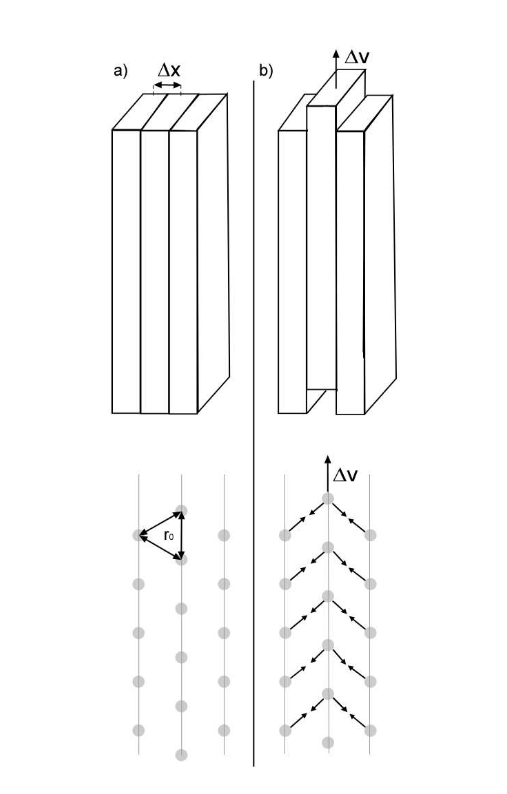
\includegraphics[width=0.5\textwidth]{./Images/FluessigkeitSchichten.png}
    \caption{Modell der Flüssigkeit als einzelne Dünne Schichten}
    \label{fig:FluessigkeitSchichten}
\end{figure}
\subsubsection*{Reynoldszahl}
\begin{list}{$\bullet$}{}
    \item Abschätzung, ob Strömung um eine Kugel laminar oder turbulent ist
    \item $R_e = \frac{v \cdot 2r \cdot \rho}{\eta}$
    \item Ungefähr: Strömung Turbulent $\Leftrightarrow$ $R_e \geq 2000$
\end{list}
\subsubsection*{Herleitung einer Formel zur Bestimmung der Viskosität}
Eine schwere Kugel sinkt durch die Summe aus Schwer- und Auftriebskraft langsam in einer Viskosen Flüssigkeit.
Hierbei tritt geschwindigkeitsabhängig Stoke'sche Reibungskraft auf. Die Kugel erreicht eine maximale Geschwindigkeit.
\begin{equation}
    \begin{split}
        F_r &= -6\pi \eta r v \\
        F_a &= -V_k \cdot \rho_f \cdot g = -\frac{4}{3}\pi r^3 \cdot \rho_f \cdot g\\
        F_g &= V_k \cdot \rho_k \cdot g = \frac{4}{3}\pi r^3 \cdot \rho_k \cdot g
    \end{split}
\end{equation}
Mit diesen Kräften folgt bei der maximalen Geschwindigkeit ($v^*$):
\begin{equation}
    \frac{4}{3}\pi r^3 \cdot g (\rho_k - \rho_f) -6\pi \eta r v^* = 0
\end{equation}
Stellt man diese Gleichung nach $\eta$ um, gilt:
\begin{equation}
    \boxed{\eta = \frac{2gr^2}{9v^*} (\rho_k - \rho_f)}
    \label{eq:viskKugel}
\end{equation}
Betrachtet man das Aufsteigen von Luftblasen mit $\rho_k \approx 0$, erhält man für $\eta$:
\begin{equation}
    \boxed{\eta = \frac{2gr^2}{9v^*} \rho_f}
    \label{eq:viskLuft}
\end{equation}

\subsection{Versuchsdurchführung}
\subsubsection{TVI: Aufstieg von Luftblasen}
In Teilversuch I wird die Viskosität eines Duschgels (\textbf{adidas ICE-DIVE}) bei zwei unterschiedlichen Temperaturen mithilfe der Aufstiegsgeschwindigkeit von Luftblasen ermittelt.
Dazu wird zunächst das Duschgel geschüttelt, um die Luftblasen zu erzeugen. Dann wird die Zeit gestoppt, die eine dieser Luftblasen benötigt, um von der unteren Höhenmarkierung bis zu der oberen Höhenmarkierung aufzusteigen zudem wird
deren Durchmesser mithilfe eines digitalen Messschiebers abgemessen.
Dieser Versuch wird 10 mal mit einem Duschgel auf Raumtemperatur wiederholt. Dann wird der gesamte Versuch nochamls für ein Duschgel durchgeführt, das zuvor mehrere Stunden im Kühlschrank gelagert wurde.
Außerdem muss noch die Dichte des Duschgels ermittelt werden. Um diese abzuschätzen, wird das Duschgel in der Flasche ins Wasser gelegt und damit aus dem Höhenunterschied des Wasser- und Duschgelpegels der 
Dichteunterschied zwischen Wasser und Duschgel abgeschätzt.

\subsection{TVII: Kufelfallviskosimeter}
In Teilversuch II wird aus einer hohen zylinderförmigen Vase ein Kugelfallviskosimeter gebaut. Hierzu wird das Duschgel aus TV I in diese Vase gefüllt. Daraufhin wird eine Metallkugel aus wenigen cm Höhe in die viskose Flüssigkeit fallen
gelassen. Der gesamte Versuch wird mithilfe der \textit{Slow-Motion}-Funktion (1/8 Geschwindigkeit) eines Smartphones gefilmt, um in der Auswertung die Sinkdauer und damit die Sinkgeschwindigkeit in der Flüssigkeit mithilfe des Videos zu bestimmen. 
Bei der verwendeten Kugel handelt es sich um eine Metallkugel aus einer Kugelbahn, deren Masse und Radius ebenfalls bestimmt wird. Der Versuch wird 5 mal wiederholt.

\newpage
\section{Versuchsprotokoll}
\subsection{Bilder der Versuchsaufbauten}
\begin{figure}[H]
    \centering
    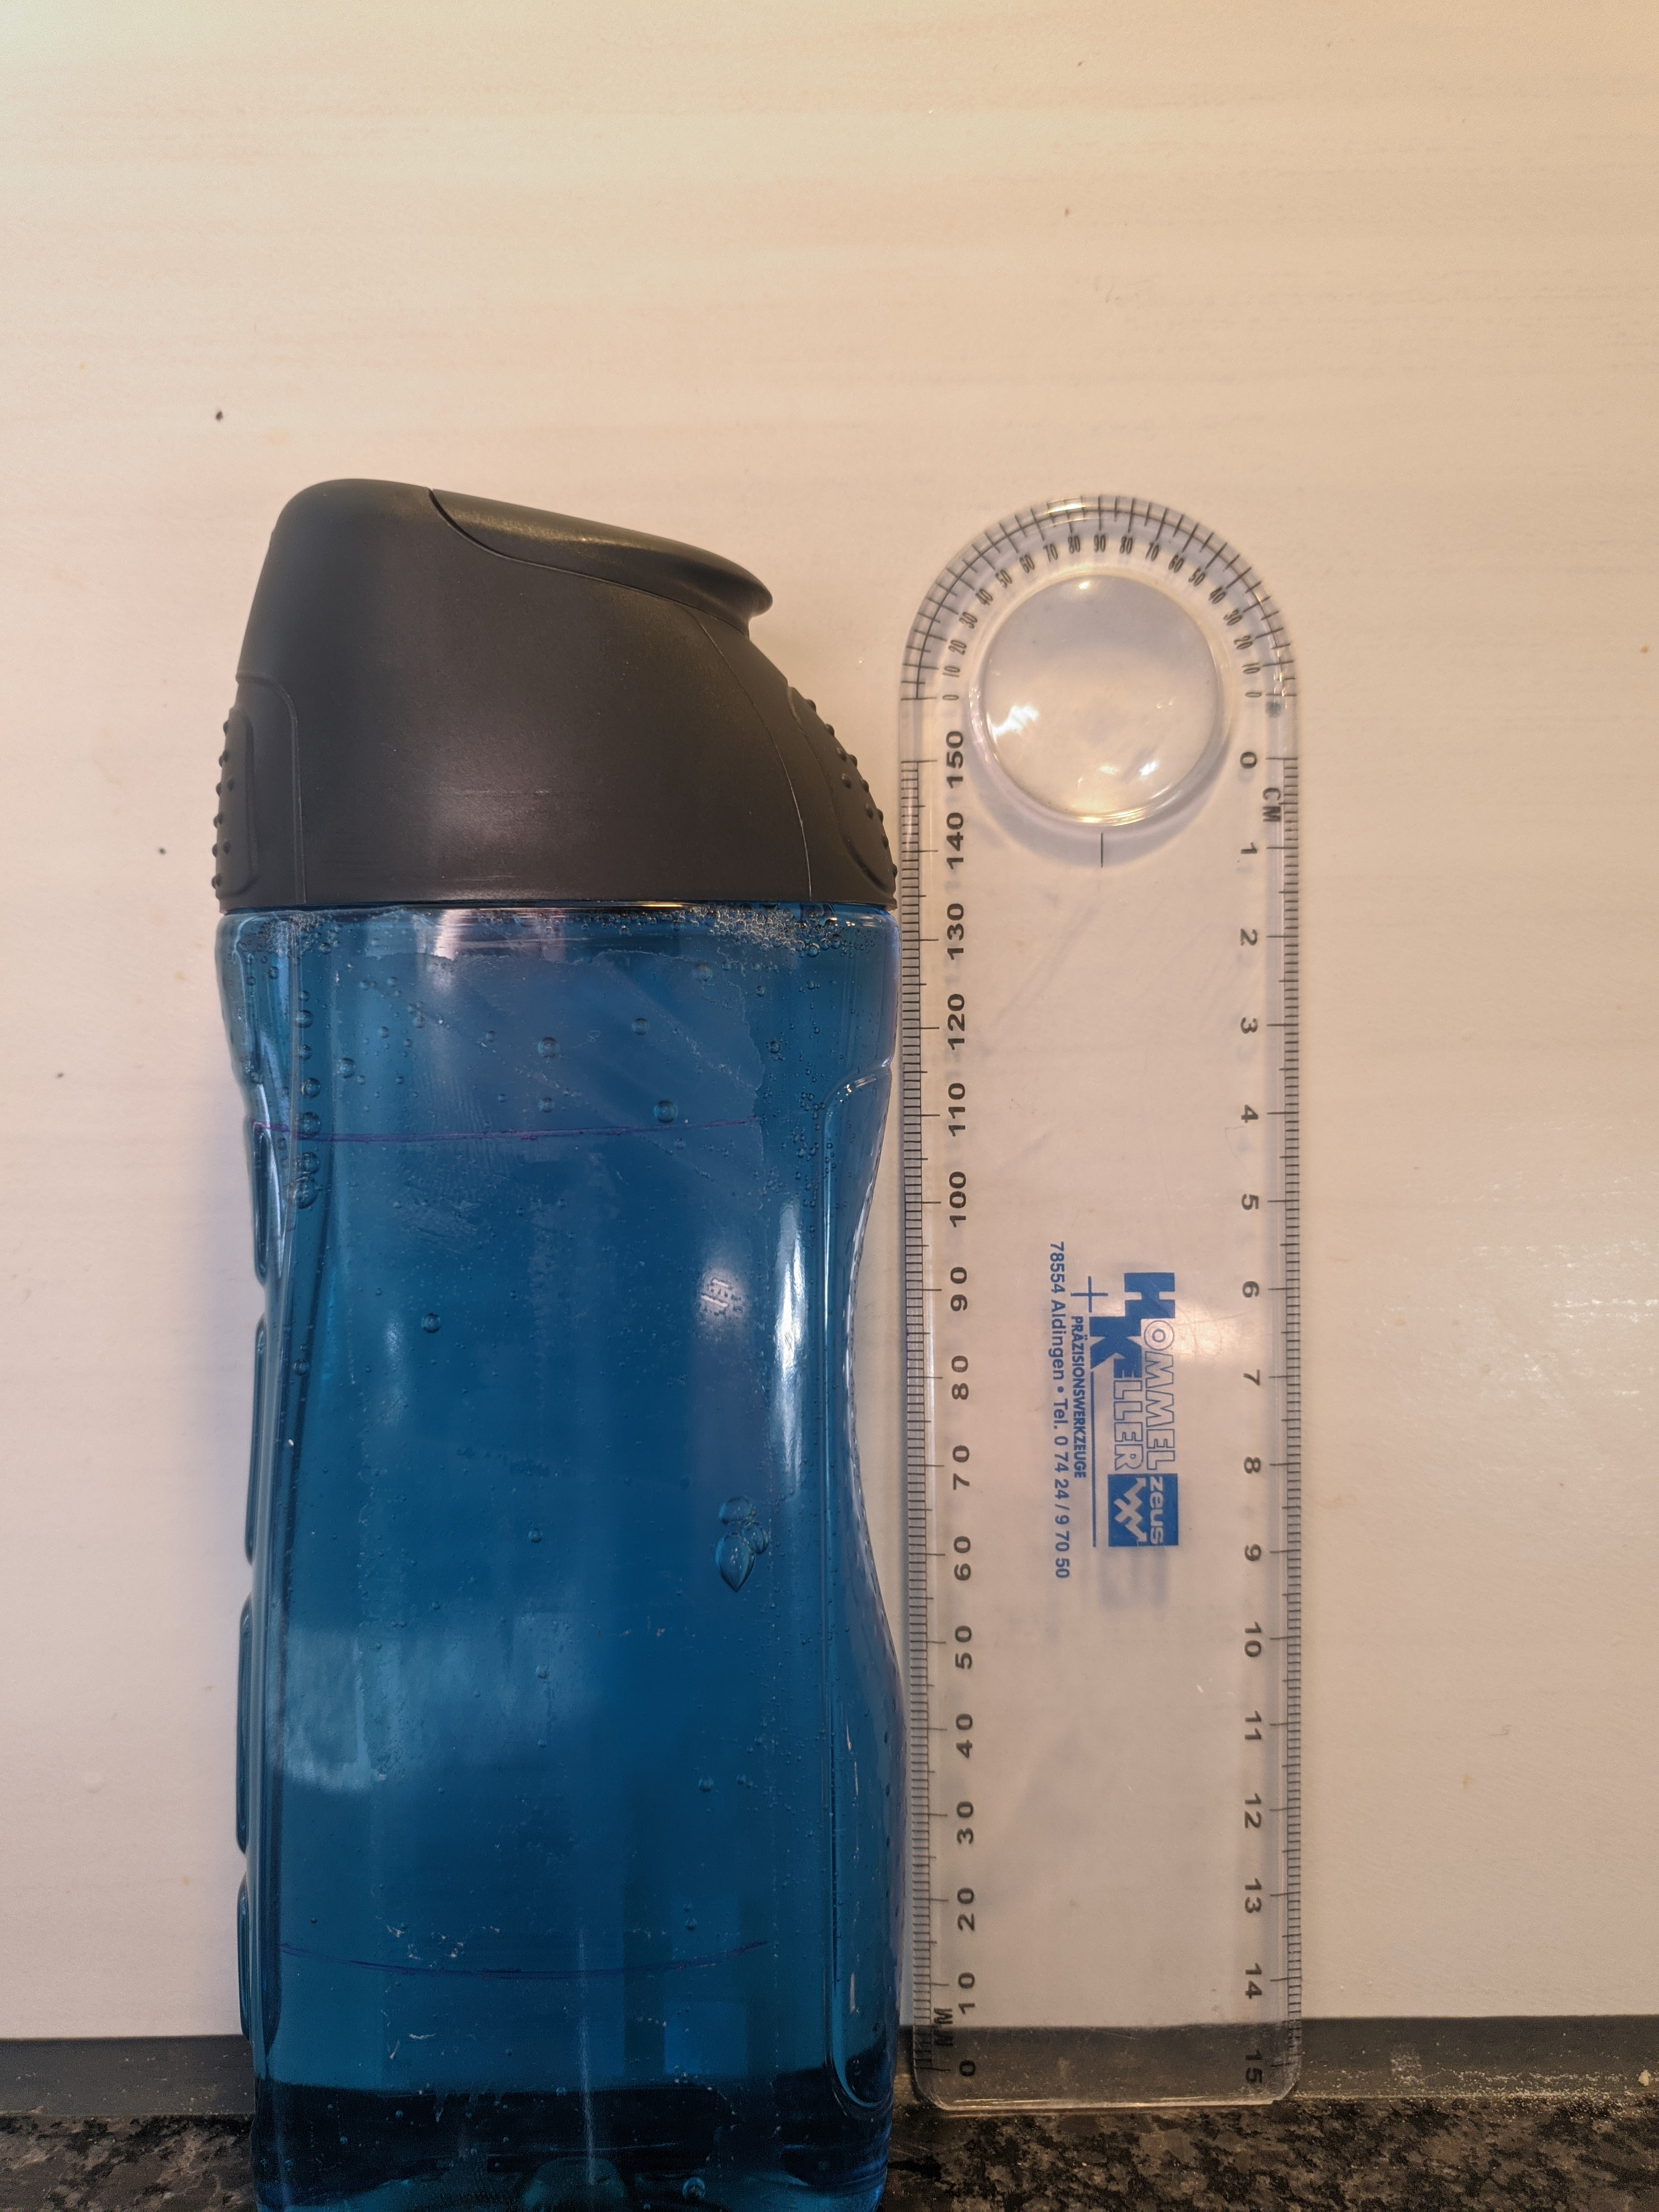
\includegraphics[width=0.35\textwidth]{./Images/VersuchsaufbauI.jpg}
    \caption{Versuchsaufbau TV I}
\end{figure}
\begin{figure}[H]
    \centering
    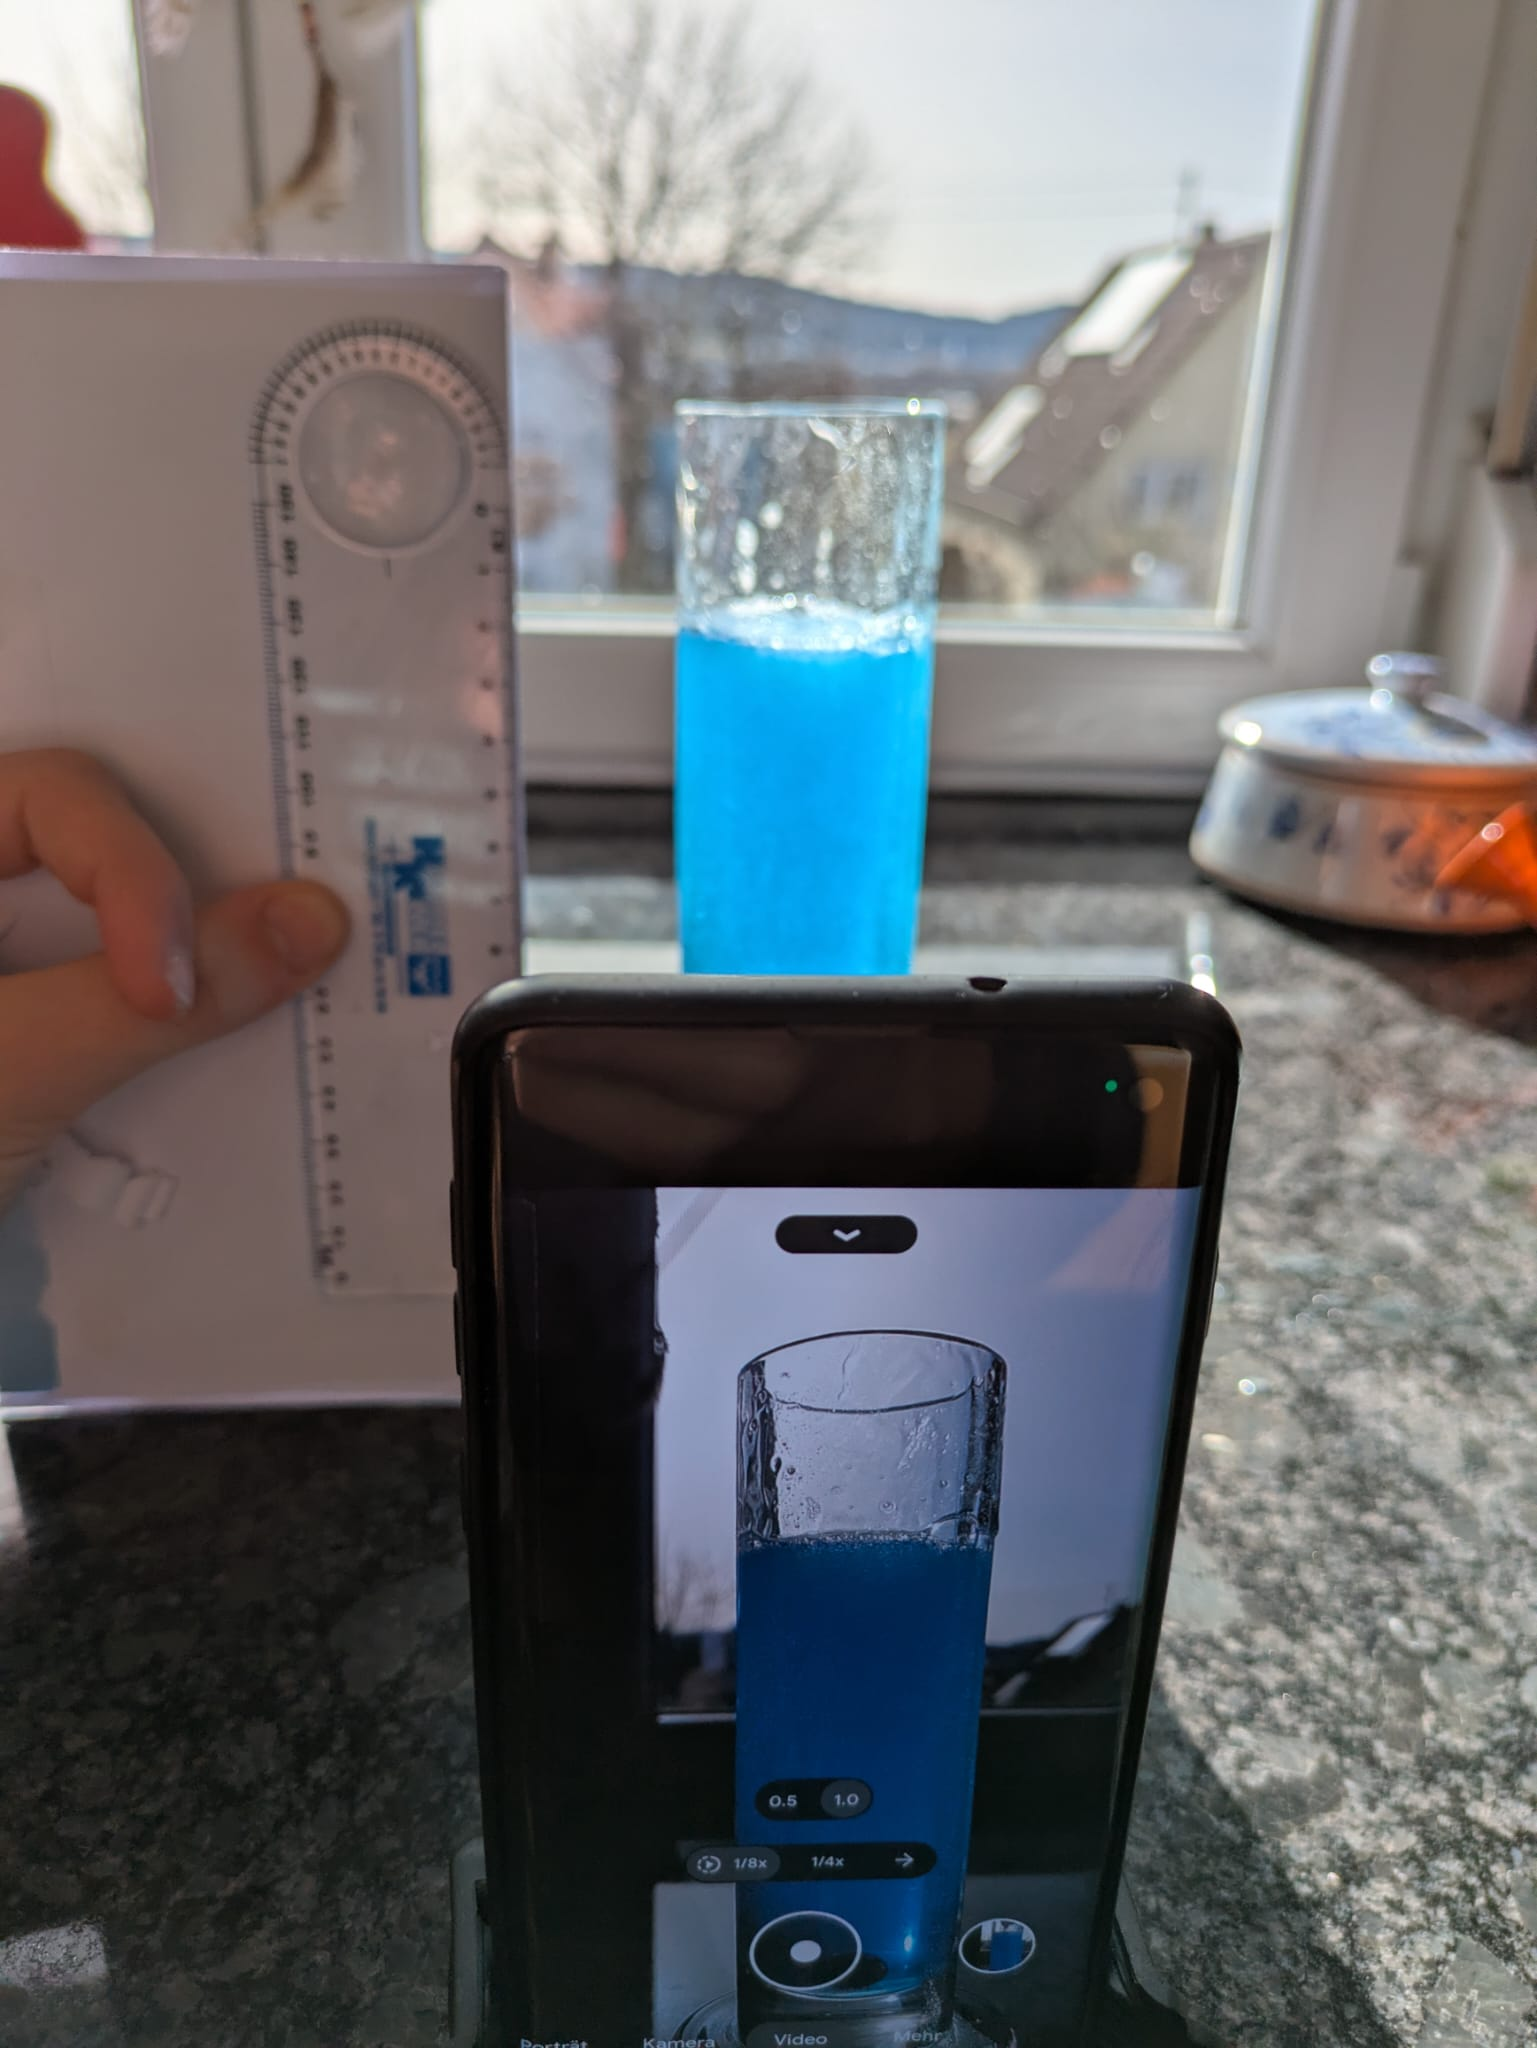
\includegraphics[width=0.35\textwidth]{./Images/VersuchsaufbauII.png}
    \caption{Versuchsaufbau TV II}
\end{figure}
\subsection{Aufschrieb}
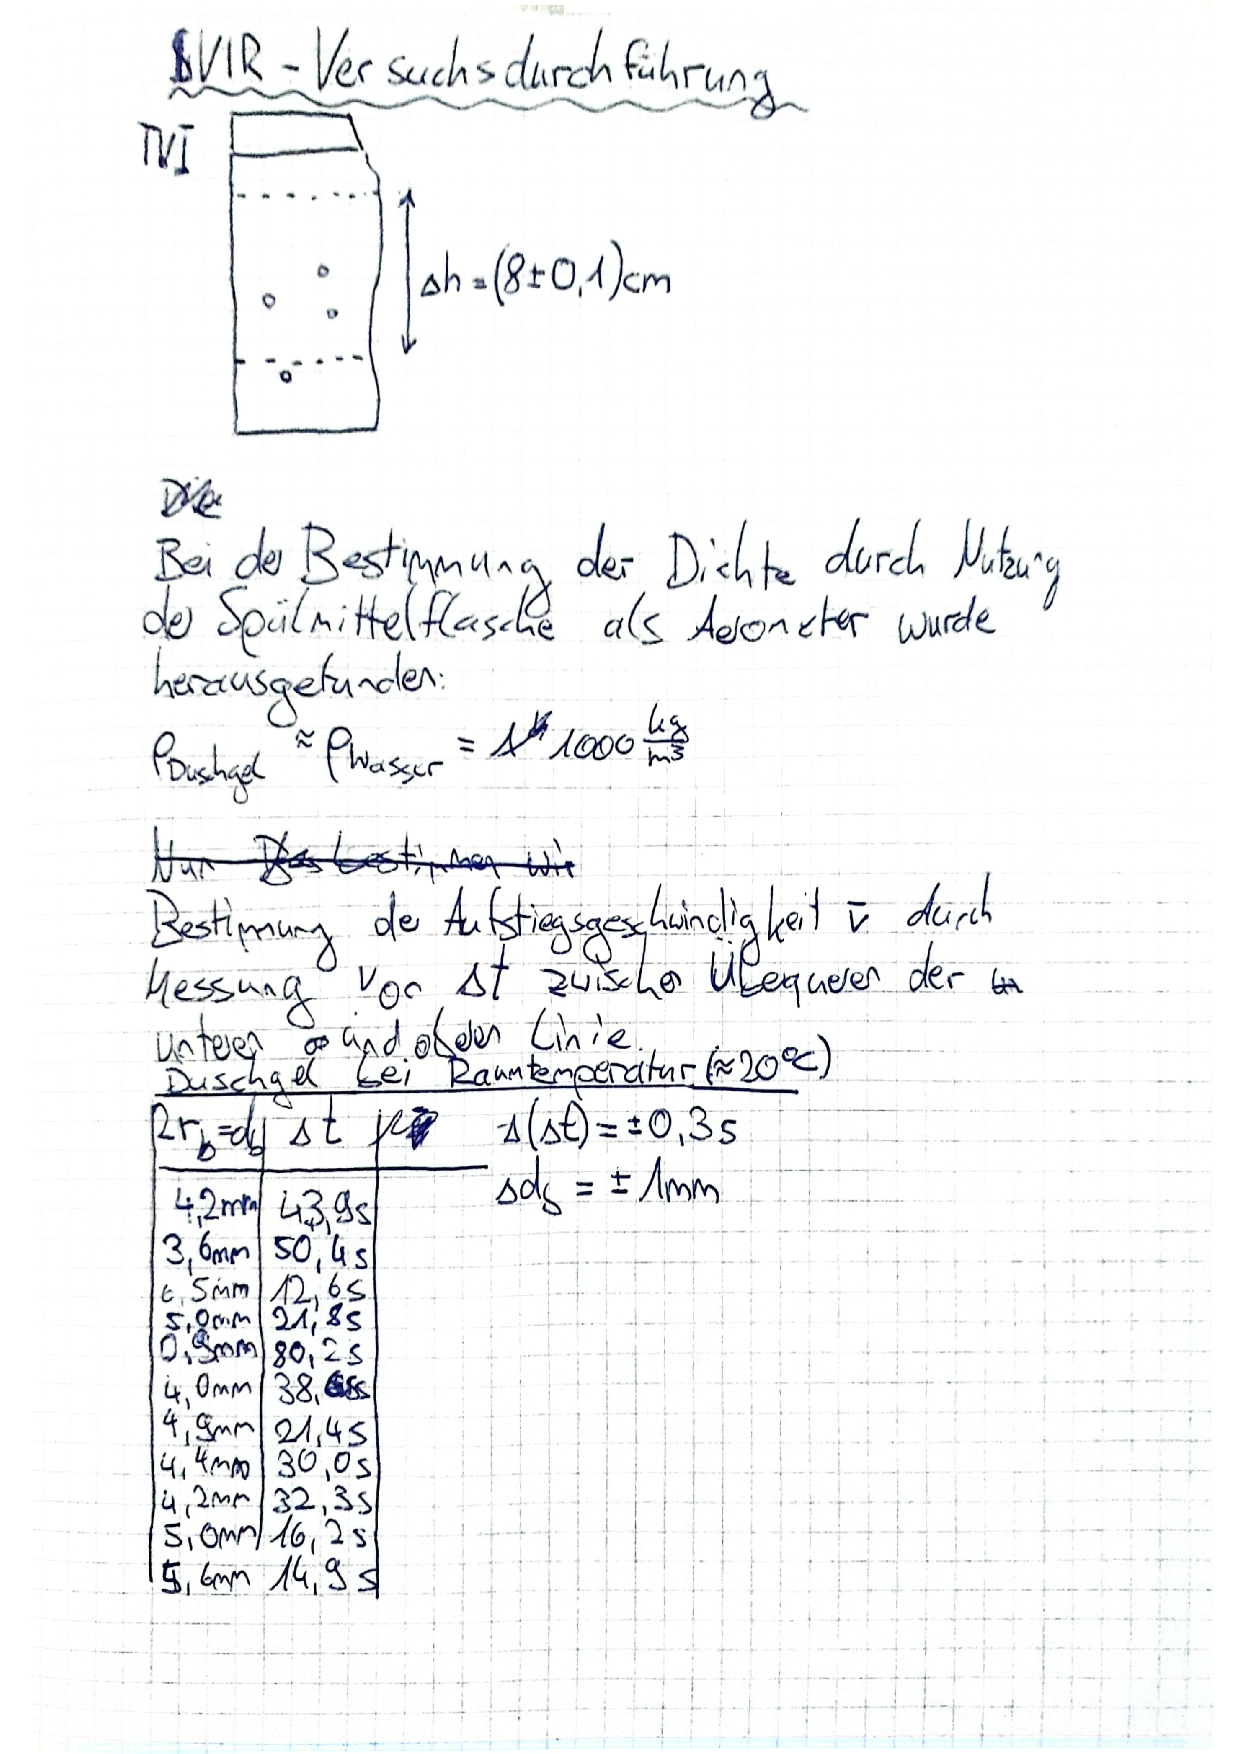
\includepdf[pages=-]{./PDFs/VIR_Versuchsdurchfuehrung.pdf}


\newpage
\chapter{Auswertung}
\section{Teilversuch I:}
\subsection{Berechnung der Viskosität}
Die Messergebnisse aus TV1 sind in den Tabellen \ref{tab:AufstiegLuftblasenRT} und \ref{tab:AufstiegLuftblasenKT}.
Die Aufstiegsgeschwindigkeiten wurden hier folgendermaßen berechnet:($v_{steig} = \frac{s}{t_{steig}}$).
Bei Raumtemperatur liegt $s$ für alle Messwerte bei $(8\pm0.1)cm$, bei Kühlschranktemperatur sind die Steighöhen jeweils gegeben.
Dies war nötig, da es sich bei Kühlschranktemperatur als sehr schwierig erwies, Luftblasen zu bilden, die unterhalb der unteren Höhenmarkierung anfangen zu steigen.
Die Viskositäten wurden jeweils mit der Formel \ref{eq:viskLuft} berechnet. (Mit $\rho_f = 1000 kg/m^3$)
\begin{table}[H]
    \centering
    \caption{Aufstiegsgeschwindigkeiten der Luftblasen bei Raumtemperatur}
    \label{tab:AufstiegLuftblasenRT}
    \begin{tabular}{c c c c}
        \hline
        Radius der Luftblase($r_k$) & Aufstiegszeit ($t_{steig}$) & Steiggeschwindigkeit ($v_{steig}$) & Viskosität ($\eta$) \\
        \hline
        $(2.1 \pm 0.5)mm$ & $(43.9 \pm 0.3)s$ & $0.182 \si{\cm} / \si{\s}$  & $5.28 \si{\Pa} \cdot \si{\s}$\\
        $(1.8 \pm 0.5)mm$ & $(50.4 \pm 0.3)s$ & $0.159 \si{\cm} / \si{\s}$  & $4.44 \si{\Pa} \cdot \si{\s}$\\
        $(3.3 \pm 0.5)mm$ & $(12.6 \pm 0.3)s$ & $0.635 \si{\cm} / \si{\s}$  & $3.74 \si{\Pa} \cdot \si{\s}$\\
        $(2.5 \pm 0.5)mm$ & $(21.8 \pm 0.3)s$ & $0.367 \si{\cm} / \si{\s}$  & $3.71\si{\Pa} \cdot \si{\s}$\\
        $(2.0 \pm 0.5)mm$ & $(38.6 \pm 0.3)s$ & $0.207 \si{\cm} / \si{\s}$  & $4.21\si{\Pa} \cdot \si{\s}$\\
        $(2.4 \pm 0.5)mm$ & $(21.4 \pm 0.3)s$ & $0.374 \si{\cm} / \si{\s}$  & $3.36\si{\Pa} \cdot \si{\s}$\\
        $(2.2 \pm 0.5)mm$ & $(30.0 \pm 0.3)s$ & $0.267 \si{\cm} / \si{\s}$  & $3.95\si{\Pa} \cdot \si{\s}$\\
        $(2.1 \pm 0.5)mm$ & $(32.3 \pm 0.3)s$ & $0.248 \si{\cm} / \si{\s}$  & $3.88\si{\Pa} \cdot \si{\s}$\\
        $(2.5 \pm 0.5)mm$ & $(16.2 \pm 0.3)s$ & $0.494 \si{\cm} / \si{\s}$  & $2.76\si{\Pa} \cdot \si{\s}$\\
        $(2.8 \pm 0.5)mm$ & $(14.5 \pm 0.3)s$ & $0.552 \si{\cm} / \si{\s}$  & $3.10\si{\Pa} \cdot \si{\s}$\\
        \hline
    \end{tabular}
\end{table}
    \begin{table}[H]
        \centering
        \caption{Aufstiegsgeschwindigkeiten der Luftblasen bei Kühlschranktemperatur}
        \label{tab:AufstiegLuftblasenKT}
        \begin{tabular}{c c c c}
            \hline
            Radius der Luftblase($r_k$) & Aufstiegszeit ($t_{steig}$) & Steiggeschwindigkeit ($v_{steig}$) & Viskosität ($\eta$) \\
            \hline
            $(2.1 \pm 0.5)mm$ & $(68.9 \pm 0.3)s$ & $0.116 \si{\cm} / \si{\s}$  & $8.28 \si{\Pa} \cdot \si{\s}$\\
            $(3.8 \pm 0.5)mm$ & $(11.9 \pm 0.3)s$ & $0.336 \si{\cm} / \si{\s}$  & $9.37 \si{\Pa} \cdot \si{\s}$\\
            $(2.8 \pm 0.5)mm$ & $(36.9 \pm 0.3)s$ & $0.217 \si{\cm} / \si{\s}$  & $7.88 \si{\Pa} \cdot \si{\s}$\\
            $(2.7 \pm 0.5)mm$ & $(14.0 \pm 0.3)s$ & $0.286 \si{\cm} / \si{\s}$  & $5.56 \si{\Pa} \cdot \si{\s}$\\
            $(1.8 \pm 0.5)mm$ & $(59.4 \pm 0.3)s$ & $0.135 \si{\cm} / \si{\s}$  & $5.24 \si{\Pa} \cdot \si{\s}$\\
            \cdashline{1-4}
            $(5.8 \pm 0.5)mm$ & $(10.8 \pm 0.3)s$ & $0.370 \si{\cm} / \si{\s}$  & $19.80 \si{\Pa} \cdot \si{\s}$\\
            $(2.5 \pm 0.5)mm$ & $(35.9 \pm 0.3)s$ & $0.111 \si{\cm} / \si{\s}$  & $12.23 \si{\Pa} \cdot \si{\s}$\\
            $(4.6 \pm 0.5)mm$ & $(12.7 \pm 0.3)s$ & $0.315 \si{\cm} / \si{\s}$  & $14.65 \si{\Pa} \cdot \si{\s}$\\
            $(6.6 \pm 0.5)mm$ & $(7.5 \pm 0.3)s$ & $0.533 \si{\cm} / \si{\s}$  & $17.81 \si{\Pa} \cdot \si{\s}$\\
            $(2.2 \pm 0.5)mm$ & $(88.6 \pm 0.3)s$ & $0.090 \si{\cm} / \si{\s}$  & $11.69 \si{\Pa} \cdot \si{\s}$\\
            \hline
        \end{tabular}
    \end{table}
\subsection{Unsicherheit der Messwerte}
Aus diesen Messwerten wird dann noch der Mittelwert sowie dessen Unsicherheit berechnet.
Während der Messung mit der Kühlschranktemperatur fiel auf, dass sich die Temperatur nach 5 Durchläufen bereits wieder stark erhöht hatte. Deshalb wurde
hier die Durchführung pausiert und das Duschgel nochmals gekühlt. Laut Tabelle unterscheiden sich die Viskositäten vor und nach der Pause stark voneinander, weshalb
diese im folgenden separat betrachet werden.

\begin{table}[H]
    \centering
    \renewcommand{\arraystretch}{3}
    \begin{tabular}{c c c c}
        Formel & $\vartheta_R$ & $\vartheta_{K1}$ & $\vartheta_{K2}$ \\
        \hline
        $\begin{aligned}
            \bar{\eta} = \frac{1}{n} \sum_{i=1}^{n} \eta_n
        \end{aligned}$ & 
        $\begin{aligned}
            \bar{\eta}_{rt} = 3.84 \si{\Pa} \cdot \si{\s}
        \end{aligned}$  & 
        $\begin{aligned}
            \bar{\eta}_{kt_1} = 7.27 \si{\Pa} \cdot \si{\s}
        \end{aligned}$ &
        $\begin{aligned}
            \bar{\eta}_{kt_2} = 15.24 \si{\Pa} \cdot \si{\s}
        \end{aligned}$
        \\
        \cdashline{1-4}
        $\begin{aligned}
            \sigma = \sqrt{\frac{1}{n-1}\sum_{i=1}^{n} (\delta \eta_i)^2}
        \end{aligned}$  & 
        $\begin{aligned}
            \sigma_{rt} = 0.711 \si{\Pa} \cdot \si{\s}
        \end{aligned}$ &
        $\begin{aligned}
            \sigma_{kt_1} = 1.792 \si{\Pa} \cdot \si{\s}
        \end{aligned}$  &
        $\begin{aligned}
            \sigma_{kt_2} = 3.51 \si{\Pa} \cdot \si{\s}
        \end{aligned}$
        \\[0.1em]
        \cdashline{1-4}
        $\begin{aligned}
            \Delta \eta = \frac{\sigma}{\sqrt{n}}
        \end{aligned}$  & 
        $\begin{aligned}
            \Delta \eta_{rt} = 0.23 \si{\Pa} \cdot \si{\s}
        \end{aligned}$ &
        $\begin{aligned}
            \Delta \eta_{kt_1} = 0.8 \si{\Pa} \cdot \si{\s}
        \end{aligned}$  &
        $\begin{aligned}
            \Delta \eta_{kt_2} = 1.6 \si{\Pa} \cdot \si{\s}
        \end{aligned}$
        \\
        \cdashline{1-4}
        $\begin{aligned}
            \eta = \bar{\eta} \pm \Delta \eta
        \end{aligned}$  & 
        $\boxed{
        \begin{aligned}
        & \eta_{rt} \\
        =& (3.84 \pm 0.23)\,\si{\Pa\cdot s}
        \end{aligned}
        }$ &
        $\boxed{
        \begin{aligned}
        &\eta_{kt_1} \\
        =& (7.3 \pm 0.8)\,\si{\Pa\cdot s}
        \end{aligned}
        }$ &
        $\boxed{
        \begin{aligned}
        &\eta_{kt_2} \\
        =& (15.2 \pm 1.6)\,\si{\Pa\cdot s}
        \end{aligned}
        }$
    \end{tabular}
\end{table}
Die bestimmten Messwerte haben eine relativ hohe Unsicherheit von ca. $\pm 10\%$.
Diese ist auf mehrere Ursachen zurückzuführen.
\subsubsection{Unsicherheit durch Zeitmessung}
Einerseits spielt die Messungenauigkeit der Zeitmessung eine Rolle für die Unsicherheit des Ergebnis. Diese setzt sich aus der Reaktionszeit beim Stoppen mit der
Stoppuhr sowie aus der Unsicherheit bei der Bestimmung des Zeitpunkts, an dem die Luftblase die Linie überquert hat zusammen. Allerdings ist diese in Relation zu den langen Aufstiegszeiten eher klein. 
\subsubsection{Unsicherheit bei der Bestimmung des Radius der Luftblasen}
Die Unsicherheit bei der Messung des Radius spielt eine deutlich bedeutendere Rolle. \\Da der Durchmesser der Blasen relativ klein ist, dieser allerdings nicht direkt mit dem Messschieber abgemessen werden kann,
muss er von außen mithilfe des Messschiebers abgeschätzt werden. Diese Schätzung hat mehrere Probleme.
Einerseits ist es ohnehin schon schwierig, den Durchmesser einer kugel mithilfe eines Messschiebers abzuschätzen, ohne diese berühren zu können. Hier spielt zum Einen 
die Perspektive mit der man auf den Messschieber und die Kugel/Blase schaut eine bedeutende Rolle, zum Anderen ist die Wahrnehmung des Durchmessers auch abhängig
vom Abstand zwischen Messschieber und Luftblase. Weil die Luftblasen nicht immer gleich weit vom Rand der Flasche sind, spielt ist auch dies nicht zu vernachlässigen. \\
Darüber hinaus kommt es durch die Krümmung der Flasche zu einer ungleichmäßigen Brechung des Lichts, so dass die Luftblase von außen ebenfalls wieder je nach Position unterschiedlich wahrgenommen wird. \\
All diese Effekte führen zu einer bereits großen Unsicherheit des Radius. Da der Radius bei der Bestimmung der Viskosität zudem quadratisch eingeht (\textit{Siehe Formel \ref{eq:viskLuft}}), wird diese 
Unsicherheit nochmals verstärkt.
\subsubsection{Unsicherheit durch Erwärmung des Duschgels}
Da die Viskosität Temperaturabhängig ist, spielt die Unsicherheit, die aufgrund der nicht konstanten Temperatur des Duschgels entsteht eine nicht zu vernachlässigungde
Rolle. Insbesondere im Versuch mit dem gekühlten Duschgel ist klar erkennbar. Hier beginnt das Duschgel sich, nachdem es aus dem Kühlschrenk genommen wurde, durch die 
höhere Außentemperatur konstant zu erwärmen. Dadurch sinkt die Viskosität des Duschgels über den Versuchsverlauf hinweg. Diese Tendenz ist in Tabelle \ref{tab:AufstiegLuftblasenKT}
klar erkennbar. \textit{(Die Messwerte sind in chronologischer Reihenfolge gegeben. Unterhalb der gestrichelten Linie beginnt der Abfall der Viskosität
erneut, da hier zwischendurch das Duschgel nochmals gekühlt wurde)}
\subsection{Systematische Fehler}
\subsubsection{Fehler durch ungenau eingezeichnete Höhenmarkierungen}
Durch ungenaues Einzeichnen der Höhenmarkierungen kommt es zu einem systematischen Fehler bei der Bestimmung der Aufstiegsgeschwindigkeit, da in den Berechnungen von
einer perfekten Höhe ausgegangen. Dieser Fehler ist allerdings im Vergleich zu den meisten anderen diskutierten Fehlern ziemlich gering.
\subsubsection{Fehler durch Beschleunigung der Luftblase}
Ein weiterer systematischer Fehler ist, dass davon ausgegangen wird, dass die Blase mit konstanter Geschwindigkeit aufsteigt. Allerdings ist dies natürlich nicht der 
Fall, da die Endgeschwindigkeit $v^*$ nur für $t\to \infty$ erreicht wird. Die Blase befindet sich also während der Geschwindigkeitsmessung noch im Beschleunigungsvorgang.
Damit ist die gemessene Durchschnittsgeschwindigkeit geringer als die theoretisch vorhergesagte. Dennoch steigt die Blase annähernd mit ihrer Endgeschwindigkeit nach oben, da der Beschleunigungsvorgang
die Blase schnell in Richtung der Endgeschwindigkeit bringt. Somit ist der hierdurch entstandene Fehler vermutlich ebenfalls relativ klein.
\subsection{Fehler durch Tropfenform}
In der Realität sind die aufsteigenden Luftblasen nicht perfekt Kugelförmig, sondern sind Tropfenförmig. Dies führt dazu, dass der horizonal gemessene Durchmesser kleiner
ist als der tatsächliche effektive Blasendurchmesser. Dieser Effekt tritt insbesondere bei großen Luftblasen auf, da diese stärker tropfenförmig sind. 
\subsection{Fehler durch Schätzung der Dichte}
Im Versuch wurde die Dichte des Duschgels nur geschätzt. Hierbei wurde u.a. die Masse der Verpackung teilweise vernachlässigt. Um diesen Fehler zu minimieren, 
könnte man eventuell ein echtes Aerometer verwenden, um die Dichte präziser zu bestimmen. Alternativ wäre auch eine Volumen- und Massemessung möglich.

\subsection{Reynoldszahl der Strömung}
Die Reynoldszahl ist durch die Formel \ref{eq:Reynoldszahl} gegeben.
\begin{equation}
    R_e = \frac{v \cdot 2r \cdot \rho}{\eta}
    \label{eq:Reynoldszahl}
\end{equation}
Die maximale Reynoldszahl, die in dem Versuch erreicht wurde errechnet man mit der Luftblase mit dem größten Radius und der höchsten 
Aufstiegsgeschwindigkeit bei Raumtemperatur (minimale Viskosität). 
\begin{equation}
    R_{e, RT} = \frac{0.635cm/s \cdot 6.6mm \cdot 1000kg/m^3}{3.84\si{\Pa \cdot \s}} = 1.09 \cdot 10^{-2}
\end{equation}
Die Reynoldszahl ist also deutlich kleiner als 2000, weshalb es sich eindeutig um eine laminare Strömung handelt.

\subsection{Vergleich der Viskosität mit Herstellerangaben}
Bei der Such nach einer Herstellerangabe zur Viskosität des Duschgels wurden leider keine Ergebnisse gefunden. Die hauptzutaten haben bei Raumtemperatur eine typische
Viskosität von $0.1-4 \si{\Pa \cdot \s}$. Bei weiterer Recherche stößt man für die Viskosität von Duschgel bei Raumtemperatur auf Werte zwischen ca. $1 \si{\Pa \cdot \s}$ und $4 \si{\Pa \cdot \s}$.
Der experimentell bestimmte Wert von $(3.84 \pm 0.23) \si{\Pa \cdot \s}$ ist also mit diesen Werten verträglich.

\subsection{Viskosität bei verschiedenen Temperaturen}
Im Versuch wurde die Viskosität für zwei verschiedene Temperaturen bestimmt.
Aus den Messwerten geht hervor, dass die Viskosität bei niedrigerer Temperatur zunimmt, da die Viskositäten für das Duschgel, das zuvor gekühlt worden war deutlich höher sind als die Viskosität bei Raumtemperatur.
Dies ist mit der Theorie vereinbar, da die Viskosität einer Flüssigkeit laut Theorie aufgrund erhöhter Molekularbewegung mit zunehmender Temperatur abnimmt. \\ 
Der große Unterschied zwischen den Messwerten für die ersten und letzten fünf Messwerte bei Kühlschranktemperatur ergibt sich vermutlich daraus, dass das Duschgel vor den ersten fünf Messungen bereits wenige Minuten vor dem Versuch aus dem Kühlschrank genommen wurde, u.a. auch,
um zunächst das Erzeugen von Blasen zu testen und um weitere Vorbereitungen, wie das Markieren der Höhenlinien zu treffen. Hierdurch war dessen Temperatur bereits deutlich höher als bei den fünf letzten Messwerten, bei welchen die Messung direkt nach 
dem herausnehmen aus dem Kühlschrank durchgeführt wurde. Dies führt zu einer deutlich höheren Viskosität bei den letzten fünf Messwerten.


\newpage
\section{Teilversuch II: Kufelfallviskosimeter}
\subsection{Berechnung der Viskosität}
In Teilversuch II wurde ein Kugelfallviskosimeter gebaut.
Folgende Fallzeiten wurden bestimmt:
\begin{equation*}
    \begin{split}
        t_1 = (0.429 \pm 0.013)s \\
        t_2 = (0.451 \pm 0.013)s \\
        t_3 = (0.440 \pm 0.013)s \\
        t_4 = (0.433 \pm 0.013)s \\
        t_5 = (0.436 \pm 0.013)s
    \end{split}
\end{equation*}
Der Mittelwert dieser Messwerte ist gegeben durch:
\begin{equation}
    \begin{split}
        \bar{t} &= \frac{1}{n} \sum_{i=1}^{n} t_n \\
                &= 0.4378s
    \end{split}
\end{equation}
Der Fehler des Messwerts kann abgeschätzt werden als:
\begin{equation}
    \begin{split}
        \Delta t &= (t_{max} - t_{min})/2 \\
                 &= (0.451-0.433)/2 \si{\s} \\
                 &= 0.009s
    \end{split}
\end{equation}
Mit dieser Berechnung ergibt sich für die bestimmten Messwerte:
\begin{equation}
    \begin{split}
        t_{fall} &= (0.438 \pm 0.009)s\\
        s_{fall} &= (70 \pm 0.5)mm \\
        r_k &= (6.39 \pm 0.02)mm \\
        m_k &= (8.50 \pm 0.14)g \\
    \end{split}
\end{equation}
Aus Strecke und Zeit ergibt sich für den Mittelwert der mittleren Fallgeschwindigkeit:
\begin{equation}
    \begin{split}
        \bar{\bar{v}}  &= \frac{s_{fall}}{t_{fall}} \\
                       &= 0.160 m/s
    \end{split}
\end{equation}
Der Fehler der mittleren Fallgeschwindigkeit ergibt sich folgendermaßen:
\begin{equation}
    \begin{split}
        \Delta \bar{v} &= \sqrt{\left(\frac{\partial v}{\partial t} \Delta t\right)^2 + \left(\frac{\partial v}{\partial s} \Delta s\right)^2} \\
                       &= \sqrt{\left(\frac{s_{fall}}{t_{fall}^2} \Delta t\right)^2 + \left(\frac{1}{t_{fall}} \Delta s\right)} \\
                       &= 0.00348 m/s \\
                       &\approx 0.004m/s
    \end{split}
\end{equation}
Also liegt die mittlere Fallgeschwindigkeit bei:
\begin{equation}
    \bar{v} = (0.160 \pm 0.004) m/s
\end{equation}
Die Dichte der Kugel ist gegeben durch:
\begin{equation}
    \begin{split}
        \bar{\rho}_k &= \frac{m_k}{V_k} \\
               &= \frac{m_k}{\frac{4}{3}\pi r_k^3} \\
               &= 7777,3 kg/m^3
    \end{split}
\end{equation}
Die Unsicherheit der Dichte ergibt sich als:
\begin{equation}
    \begin{split}
        \Delta \bar{v} &= \sqrt{\left(\frac{\partial \rho}{\partial m} \Delta m\right)^2 + \left(\frac{\partial rho}{\partial r} \Delta r\right)^2} \\
                       &= \sqrt{\left(\frac{\Delta m}{\frac{4}{3} \pi r_k^3}\right)^2 + \left(\frac{9m_k}{4\pi r_k^4} \Delta r\right)^2} \\
                       &\approx 150 kg/m^3
    \end{split}
\end{equation}
Somit liegt die Dichte der Metallkugel bei:
\begin{equation}
    \rho_k = (7.78 \pm 0.15) \cdot 10^3 kg/m^3
\end{equation}
Die Dichte des Duschgels wurde geschätzt auf:
\begin{equation}
    \rho_f = (1.0 \pm 0.2) \cdot 10^3 kg/m^3
\end{equation}
Nun kann aus diesen Werten die Viskosität berechnet werden:
\begin{equation}
    \begin{split}
        \bar{\eta} &= \frac{2gr_k^2}{9\bar{v}}\left(\rho_k - \rho_f\right) \\
                   &= 3.77 \si{\Pa \cdot \s}
    \end{split}
\end{equation}
Die relative Unsicherheit von $\eta$ ergibt sich aus:
\begin{equation}
    \begin{split}
        \frac{\Delta \eta}{\eta} &= \frac{1}{\eta} \sqrt{  \left(\frac{\partial \eta}{\partial r} \Delta r\right)^2
                                                        + \left(\frac{\partial \eta}{\partial v} \Delta v\right)^2
                                                        + \left(\frac{\partial \eta}{\partial \rho_k} \Delta \rho_k \right)^2
                                                        + \left(\frac{\partial \eta}{\partial \rho_f} \Delta \rho_f \right)^2} \\
                                 &= \frac{1}{\eta} \sqrt{\left(\frac{2\eta}{r} \Delta r\right)^2
                                                        + \left(\frac{\eta}{\bar{v}} \Delta \bar{v}\right)^2
                                                        + \left(\frac{\eta}{\rho_k - \rho_f} \cdot \Delta \rho_k\right)^2
                                                        + \left(\frac{\eta}{\rho_k - \rho_f} \cdot \Delta \rho_f\right)^2} \\
                                 &= \sqrt{\left(2\frac{\Delta r}{r}\right)^2 
                                                        + \left(\frac{\Delta v}{v}\right)^2 
                                                        + \left(\frac{\Delta \rho_k}{\rho_k - \rho_f}\right)^2
                                                        + \left(\frac{\Delta \rho_f}{\rho_k - \rho_f}\right)^2}
    \end{split}
\end{equation}
Einsetzen der Werte liefert:
\begin{eqnarray}
    \frac{\Delta \eta}{\eta} = 0.0450
\end{eqnarray}
Somit liegt die Viskosität bei:
\begin{equation}
    \begin{split}
        \eta &= \bar{\eta} \pm \frac{\Delta \eta}{\eta} \bar{\eta}\\
             &= (3.77 \pm 0.0450 \cdot 3.77) \si{\Pa \cdot \s} \\
             &= (3.77 \pm 0.17)\si{\Pa \cdot \s}
    \end{split}
\end{equation}
Wieder kann nun die Reynolds Zahl bestimmt werden:
\begin{equation}
    \begin{split}
        R_e &= \frac{v \cdot 2r \cdot \rho_f}{\eta} \\
            &= \frac{0.160\si{\m/s} \cdot 0.01278\si{\m} \cdot 1000\si{kg/m^3}}{3.77 \si{\Pa \cdot \s}} \\
            &= 0.542
    \end{split}
\end{equation}
Auch hier liegt die Reynoldszahl weit unter 2000, somit handelt es sich eindeutig um eine laminare Strömung.
\subsection{Ergebnisdiskussion}
Die durch das Kugelfallviskosimeter bestimmte Viskosität von $\eta_2 = (3.77 \pm 0.17)\si{\Pa \cdot \s}$ stimmt im Rahmen der Unsicherheit mit dem Ergebnis bei Raumtemperatur aus 
TV I ($\eta_1 = (3.84 \pm 0.23) \si{\Pa \cdot \s}$) überein. Somit ist das Ergebnis gleichermaßen mit den im Internet gegebenen Angaben verträglich.


\definecolor{codegreen}{rgb}{0,0.6,0}
\definecolor{codegray}{rgb}{0.5,0.5,0.5}
\definecolor{codepurple}{rgb}{0.58,0,0.82}
\definecolor{backcolour}{rgb}{0.95,0.95,0.92}

\lstdefinestyle{matlab}{
    backgroundcolor=\color{backcolour},   
    commentstyle=\color{codegreen},
    keywordstyle=\color{magenta},
    numberstyle=\tiny\color{codegray},
    stringstyle=\color{codepurple},
    basicstyle=\ttfamily\footnotesize,
    breakatwhitespace=false,         
    breaklines=true,                 
    captionpos=b,                    
    keepspaces=true,                 
    numbers=left,                    
    numbersep=5pt,                  
    showspaces=false,                
    showstringspaces=false,
    showtabs=false,                  
    tabsize=2
}

\end{document}
